\documentclass[10pt,a4paper]{article}
\usepackage{tikz}
\usetikzlibrary{matrix,calc}
\usepackage{multirow}
\usepackage[utf8]{inputenc}
\usepackage[spanish]{babel}
\usepackage{amsmath}
\usepackage{amsfonts}
\usepackage{amssymb}
\usepackage{graphicx}
\usepackage{float}
\usepackage[left=2cm,right=2cm,top=2cm,bottom=2cm]{geometry}
\usepackage{circuitikz}
\usepackage{tikz-timing}
\usetikztiminglibrary[rising arrows]{clockarrows}
\usepackage{pgfplots}
\pgfplotsset{compat=1.15}
\usepackage{listings}
\usepackage[export]{adjustbox}
\usepackage{graphicx,wrapfig,lipsum}
\usepackage{booktabs}
\usepackage[skip=0pt]{caption}
\captionsetup[figure]{font=small,labelfont=small}


\usetikzlibrary{matrix,calc}

%isolated term
%#1 - Optional. Space between node and grouping line. Default=0
%#2 - node
%#3 - filling color
\newcommand{\implicantsol}[3][0]{
    \draw[rounded corners=3pt, fill=#3, opacity=0.3] ($(#2.north west)+(135:#1)$) rectangle ($(#2.south east)+(-45:#1)$);
    }


%internal group
%#1 - Optional. Space between node and grouping line. Default=0
%#2 - top left node
%#3 - bottom right node
%#4 - filling color
\newcommand{\implicant}[4][0]{
    \draw[rounded corners=3pt, fill=#4, opacity=0.3] ($(#2.north west)+(135:#1)$) rectangle ($(#3.south east)+(-45:#1)$);
    }

%group lateral borders
%#1 - Optional. Space between node and grouping line. Default=0
%#2 - top left node
%#3 - bottom right node
%#4 - filling color
\newcommand{\implicantcostats}[4][0]{
    \draw[rounded corners=3pt, fill=#4, opacity=0.3] ($(rf.east |- #2.north)+(90:#1)$)-| ($(#2.east)+(0:#1)$) |- ($(rf.east |- #3.south)+(-90:#1)$);
    \draw[rounded corners=3pt, fill=#4, opacity=0.3] ($(cf.west |- #2.north)+(90:#1)$) -| ($(#3.west)+(180:#1)$) |- ($(cf.west |- #3.south)+(-90:#1)$);
}

%group top-bottom borders
%#1 - Optional. Space between node and grouping line. Default=0
%#2 - top left node
%#3 - bottom right node
%#4 - filling color
\newcommand{\implicantdaltbaix}[4][0]{
    \draw[rounded corners=3pt, fill=#4, opacity=0.3] ($(cf.south -| #2.west)+(180:#1)$) |- ($(#2.south)+(-90:#1)$) -| ($(cf.south -| #3.east)+(0:#1)$);
    \draw[rounded corners=3pt, fill=#4, opacity=0.3] ($(rf.north -| #2.west)+(180:#1)$) |- ($(#3.north)+(90:#1)$) -| ($(rf.north -| #3.east)+(0:#1)$);
}

%group corners
%#1 - Optional. Space between node and grouping line. Default=0
%#2 - filling color
\newcommand{\implicantcantons}[2][0]{
    \draw[rounded corners=3pt, opacity=.3] ($(rf.east |- 0.south)+(-90:#1)$) -| ($(0.east |- cf.south)+(0:#1)$);
    \draw[rounded corners=3pt, opacity=.3] ($(rf.east |- 8.north)+(90:#1)$) -| ($(8.east |- rf.north)+(0:#1)$);
    \draw[rounded corners=3pt, opacity=.3] ($(cf.west |- 2.south)+(-90:#1)$) -| ($(2.west |- cf.south)+(180:#1)$);
    \draw[rounded corners=3pt, opacity=.3] ($(cf.west |- 10.north)+(90:#1)$) -| ($(10.west |- rf.north)+(180:#1)$);
    \fill[rounded corners=3pt, fill=#2, opacity=.3] ($(rf.east |- 0.south)+(-90:#1)$) -|  ($(0.east |- cf.south)+(0:#1)$) [sharp corners] ($(rf.east |- 0.south)+(-90:#1)$) |-  ($(0.east |- cf.south)+(0:#1)$) ;
    \fill[rounded corners=3pt, fill=#2, opacity=.3] ($(rf.east |- 8.north)+(90:#1)$) -| ($(8.east |- rf.north)+(0:#1)$) [sharp corners] ($(rf.east |- 8.north)+(90:#1)$) |- ($(8.east |- rf.north)+(0:#1)$) ;
    \fill[rounded corners=3pt, fill=#2, opacity=.3] ($(cf.west |- 2.south)+(-90:#1)$) -| ($(2.west |- cf.south)+(180:#1)$) [sharp corners]($(cf.west |- 2.south)+(-90:#1)$) |- ($(2.west |- cf.south)+(180:#1)$) ;
    \fill[rounded corners=3pt, fill=#2, opacity=.3] ($(cf.west |- 10.north)+(90:#1)$) -| ($(10.west |- rf.north)+(180:#1)$) [sharp corners] ($(cf.west |- 10.north)+(90:#1)$) |- ($(10.west |- rf.north)+(180:#1)$) ;
}

%Empty Karnaugh map 4x4
\newenvironment{Karnaugh}%
{
\begin{tikzpicture}[baseline=(current bounding box.north),scale=0.8]
\draw (0,0) grid (4,4);
\draw (0,4) -- node [pos=0.7,above right,anchor=south west] {cd} node [pos=0.7,below left,anchor=north east] {ab} ++(135:1);
%
\matrix (mapa) [matrix of nodes,
        column sep={0.8cm,between origins},
        row sep={0.8cm,between origins},
        every node/.style={minimum size=0.3mm},
        anchor=8.center,
        ampersand replacement=\&] at (0.5,0.5)
{
                       \& |(c00)| 00         \& |(c01)| 01         \& |(c11)| 11         \& |(c10)| 10         \& |(cf)| \phantom{00} \\
|(r00)| 00             \& |(0)|  \phantom{0} \& |(1)|  \phantom{0} \& |(3)|  \phantom{0} \& |(2)|  \phantom{0} \&                     \\
|(r01)| 01             \& |(4)|  \phantom{0} \& |(5)|  \phantom{0} \& |(7)|  \phantom{0} \& |(6)|  \phantom{0} \&                     \\
|(r11)| 11             \& |(12)| \phantom{0} \& |(13)| \phantom{0} \& |(15)| \phantom{0} \& |(14)| \phantom{0} \&                     \\
|(r10)| 10             \& |(8)|  \phantom{0} \& |(9)|  \phantom{0} \& |(11)| \phantom{0} \& |(10)| \phantom{0} \&                     \\
|(rf) | \phantom{00}   \&                    \&                    \&                    \&                    \&                     \\
};
}%
{
\end{tikzpicture}
}

%Empty Karnaugh map 2x4
\newenvironment{Karnaughvuit}%
{
\begin{tikzpicture}[baseline=(current bounding box.north),scale=0.8]
\draw (0,0) grid (4,2);
\draw (0,2) -- node [pos=0.7,above right,anchor=south west] {bc} node [pos=0.7,below left,anchor=north east] {a} ++(135:1);
%
\matrix (mapa) [matrix of nodes,
        column sep={0.8cm,between origins},
        row sep={0.8cm,between origins},
        every node/.style={minimum size=0.3mm},
        anchor=4.center,
        ampersand replacement=\&] at (0.5,0.5)
{
                      \& |(c00)| 00         \& |(c01)| 01         \& |(c11)| 11         \& |(c10)| 10         \& |(cf)| \phantom{00} \\
|(r00)| 0             \& |(0)|  \phantom{0} \& |(1)|  \phantom{0} \& |(3)|  \phantom{0} \& |(2)|  \phantom{0} \&                     \\
|(r01)| 1             \& |(4)|  \phantom{0} \& |(5)|  \phantom{0} \& |(7)|  \phantom{0} \& |(6)|  \phantom{0} \&                     \\
|(rf) | \phantom{00}  \&                    \&                    \&                    \&                    \&                     \\
};
}%
{
\end{tikzpicture}
}

%Empty Karnaugh map 2x2
\newenvironment{Karnaughquatre}%
{
\begin{tikzpicture}[baseline=(current bounding box.north),scale=0.8]
\draw (0,0) grid (2,2);
\draw (0,2) -- node [pos=0.7,above right,anchor=south west] {b} node [pos=0.7,below left,anchor=north east] {a} ++(135:1);
%
\matrix (mapa) [matrix of nodes,
        column sep={0.8cm,between origins},
        row sep={0.8cm,between origins},
        every node/.style={minimum size=0.3mm},
        anchor=2.center,
        ampersand replacement=\&] at (0.5,0.5)
{
          \& |(c00)| 0          \& |(c01)| 1  \\
|(r00)| 0 \& |(0)|  \phantom{0} \& |(1)|  \phantom{0} \\
|(r01)| 1 \& |(2)|  \phantom{0} \& |(3)|  \phantom{0} \\
};
}%
{
\end{tikzpicture}
}

%Defines 8 or 16 values (0,1,X)
\newcommand{\contingut}[1]{%
\foreach \x [count=\xi from 0]  in {#1}
     \path (\xi) node {\x};
}

%Places 1 in listed positions
\newcommand{\minterms}[1]{%
    \foreach \x in {#1}
        \path (\x) node {1};
}

%Places 0 in listed positions
\newcommand{\maxterms}[1]{%
    \foreach \x in {#1}
        \path (\x) node {0};
}

%Places X in listed positions
\newcommand{\indeterminats}[1]{%
    \foreach \x in {#1}
        \path (\x) node {X};
}
\newenvironment{KarnaughTP3}%
{
\begin{tikzpicture}[baseline=(current bounding box.north),scale=0.8]
\draw (0,0) grid (4,4);
\draw (0,4) -- node [pos=0.9,above right,anchor=south west] {$Q_1 Q_0$} node [pos=0.7,below left,anchor=north east] {$W Q_2$} ++(135:1);
%
\matrix (mapa) [matrix of nodes,
        column sep={0.8cm,between origins},
        row sep={0.8cm,between origins},
        every node/.style={minimum size=0.3mm},
        anchor=8.center,
        ampersand replacement=\&] at (0.5,0.5)
{
                       \& |(c00)| 00         \& |(c01)| 01         \& |(c11)| 11         \& |(c10)| 10         \& |(cf)| \phantom{00} \\
|(r00)| 00             \& |(0)|  \phantom{0} \& |(1)|  \phantom{0} \& |(3)|  \phantom{0} \& |(2)|  \phantom{0} \&                     \\
|(r01)| 01             \& |(4)|  \phantom{0} \& |(5)|  \phantom{0} \& |(7)|  \phantom{0} \& |(6)|  \phantom{0} \&                     \\
|(r11)| 11             \& |(12)| \phantom{0} \& |(13)| \phantom{0} \& |(15)| \phantom{0} \& |(14)| \phantom{0} \&                     \\
|(r10)| 10             \& |(8)|  \phantom{0} \& |(9)|  \phantom{0} \& |(11)| \phantom{0} \& |(10)| \phantom{0} \&                     \\
|(rf) | \phantom{00}   \&                    \&                    \&                    \&                    \&                     \\
};
}%
{
\end{tikzpicture}
}

\newenvironment{KarnaughvuiteTP3}%
{
\begin{tikzpicture}[baseline=(current bounding box.north),scale=0.8]
\draw (0,0) grid (4,2);
\draw (0,2) -- node [pos=0.9,above right,anchor=south west] {$Q_1Q_0$} node [pos=0.7,below left,anchor=north east] {$W$} ++(135:1);
%
\matrix (mapa) [matrix of nodes,
        column sep={0.8cm,between origins},
        row sep={0.8cm,between origins},
        every node/.style={minimum size=0.3mm},
        anchor=4.center,
        ampersand replacement=\&] at (0.5,0.5)
{
                      \& |(c00)| 00         \& |(c01)| 01         \& |(c11)| 11         \& |(c10)| 10         \& |(cf)| \phantom{00} \\
|(r00)| 0             \& |(0)|  \phantom{0} \& |(1)|  \phantom{0} \& |(3)|  \phantom{0} \& |(2)|  \phantom{0} \&                     \\
|(r01)| 1             \& |(4)|  \phantom{0} \& |(5)|  \phantom{0} \& |(7)|  \phantom{0} \& |(6)|  \phantom{0} \&                     \\
|(rf) | \phantom{00}  \&                    \&                    \&                    \&                    \&                     \\
};
}%
{
\end{tikzpicture}
}

\begin{document}

Se nos pidi\'o realizar una m\'aquina de Moore y una de Mealy que puedan detectar la secuencia 1-1-0-1 y avise en la salida al detectarla. Para esto tuvimos en cuenta que cuando termina la secuencia y es detectada se toma el \'ultimo 1 de la secuencia como el primero de la siguiente secuencia en caso de que ocurran 2 secuencias seguidas, la cual ser\'ia 1-1-0-1-1-0-1. Primero diseñamos un diagrama de estados basándonos en la m\'aquina de Moore, donde tendremos 5 estados. El estado A es el caso base donde se recibió un 0 fuera de la secuencia pedida, el estado B es el caso donde se recibió el primer 1, el estado C es el caso donde se recibe el segundo 1, el estado D donde se recibe la secuencia 1-1-0 y el estado E es cuando se recibe la secuencia completa. 
El diagrama queda de la siguiente manera:

\begin{figure}[hbtp]
	\centering
		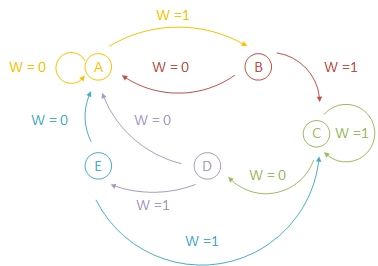
\includegraphics[scale=1]{diagestmoore.jpg}
	\caption{Diagrama de Estados - Máquina de Moore}
\end{figure}



\begin{figure}[H]
\begin{center}
\begin{tabular}{c|c|c|c|}
\cline{2-4}
\textbf{} & \textbf{W = 0} & \textbf{W = 1} & \textbf{Z} \\ \hline
\multicolumn{1}{|c|}{\textbf{A$_{000}$}} & \textbf{A} & \textbf{B} & \textbf{0} \\ \hline
\multicolumn{1}{|c|}{\textbf{B$_{001}$}} & \textbf{A} & \textbf{C} & \textbf{0} \\ \hline
\multicolumn{1}{|c|}{\textbf{C$_{010}$}} & \textbf{D} & \textbf{A} & \textbf{0} \\ \hline
\multicolumn{1}{|c|}{\textbf{D$_{011}$}} & \textbf{A} & \textbf{E} & \textbf{0} \\ \hline
\multicolumn{1}{|c|}{\textbf{E$_{100}$}} & \textbf{A} & \textbf{C} & \textbf{1} \\ \hline
\end{tabular}
\caption{Transiciones - Máquina de Moore} 
\label{2_fig1}
\end{center}
\end{figure}
	
	\begin{figure}[H]
		\begin{center}
		\begin{KarnaughTP3}
		\contingut{0,0,1,0,0,X,X,X,1,0,0,0,0,X,X,X}
		\implicant{2}{6}{red}
		\implicant{8}{8}{blue}
		\end{KarnaughTP3}
		\end{center}
		\caption{$Q_{0_{t+1}}$ Máq. de Moore} 
		\label{2_fig2}
	\end{figure}

	\begin{figure}[H]
		\begin{center}
		\begin{KarnaughTP3}
		\contingut{0,0,1,0,0,X,X,X,0,1,0,0,1,X,X,X}
		\implicant{2}{6}{orange}
		\implicant{13}{9}{green}
		\implicant{12}{14}{red}
		\end{KarnaughTP3}
		\end{center}
		\caption{$Q_{1_{t+1}}$ Máq. de Moore} 
		\label{2_fig3}
	\end{figure}

	\begin{figure}[H]
		\begin{center}
		\begin{KarnaughTP3}
		\contingut{0,0,0,0,0,X,X,X,0,0,0,1,0,X,X,X}
		\implicant{11}{11}{red}
		\end{KarnaughTP3}
		\end{center}
		\caption{$Q_{2_{t+1}}$ Máq. de Moore} 
		\label{2_fig4}
	\end{figure}
	
	\begin{figure}[H]
		\begin{center}
		\begin{KarnaughvuiteTP3}
		\minterms{4}
		\maxterms{0,1,2,3}
		\indeterminats{5,6,7}
		\implicant{4}{4}{orange}
		\end{KarnaughvuiteTP3}
		\end{center}
		\caption{$Z$: Salida - Máq. de Moore} 
		\label{2_fig5}
	\end{figure}
	
\begin{figure}[H]
\begin{center}
\begin{tabular}{|c|c|c|c|c|}
\hline
\multirow{2}{*}{\textbf{\begin{tabular}[c]{@{}c@{}}Estado\\ Actual\end{tabular}}} & \multicolumn{2}{c|}{\textbf{\begin{tabular}[c]{@{}c@{}}Estado\\ Siguiente\end{tabular}}} & \multicolumn{2}{c|}{\textbf{Salida: Z}} \\ \cline{2-5} 
 & \textbf{W = 0} & \textbf{W = 1} & \textbf{W = 0} & \textbf{W = 1} \\ \hline
\textbf{A$_{000}$} & \textbf{A} & \textbf{B} & \textbf{0} & \textbf{0} \\ \hline
\textbf{B$_{001}$} & \textbf{A} & \textbf{C} & \textbf{0} & \textbf{0} \\ \hline
\textbf{C$_{010}$} & \textbf{D} & \textbf{A} & \textbf{0} & \textbf{0} \\ \hline
\textbf{D$_{011}$} & \textbf{A} & \textbf{B} & \textbf{0} & \textbf{1} \\ \hline
\end{tabular}
\caption{Transiciones - Máquina de Mealy} 
\label{2_fig6}
\end{center}
\end{figure}

\begin{figure}[H]
\begin{center}
\begin{tabular}{|c|c|c|c|c|c|c|c|}
\hline
\multicolumn{2}{|c|}{\multirow{2}{*}{\textbf{\begin{tabular}[c]{@{}c@{}}Estado\\ Actual\end{tabular}}}} & \multicolumn{4}{c|}{\textbf{Estado Siguiente}} & \multicolumn{2}{c|}{\multirow{2}{*}{\textbf{Salida: Z}}} \\ \cline{3-6}
\multicolumn{2}{|c|}{} & \multicolumn{2}{c|}{\textbf{W = 0}} & \multicolumn{2}{c|}{\textbf{W = 1}} & \multicolumn{2}{c|}{} \\ \hline
\textbf{Q1} & \textbf{Q0} & \textbf{Q1T+1} & \textbf{Q0T+1} & \textbf{Q1T+1} & \textbf{Q0T+1} & \textbf{W = 0} & \textbf{W = 1} \\ \hline
\textbf{0} & \textbf{0} & \textbf{0} & \textbf{0} & \textbf{0} & \textbf{1} & \textbf{0} & \textbf{0} \\ \hline
\textbf{0} & \textbf{1} & \textbf{0} & \textbf{0} & \textbf{1} & \textbf{0} & \textbf{0} & \textbf{0} \\ \hline
\textbf{1} & \textbf{0} & \textbf{1} & \textbf{1} & \textbf{0} & \textbf{0} & \textbf{0} & \textbf{0} \\ \hline
\textbf{1} & \textbf{1} & \textbf{0} & \textbf{0} & \textbf{0} & \textbf{1} & \textbf{0} & \textbf{1} \\ \hline
\end{tabular}
\caption{Máquina de Mealy} 
\label{2_fig7}
\end{center}
\end{figure}

	\begin{figure}[H]
		\begin{center}
		\begin{KarnaughvuiteTP3}
		\minterms{2,4,7}
		\maxterms{0,1,3,5,6}
		%\indeterminats{2,5}
		\implicant{2}{2}{green}
		\implicant{4}{4}{red}
		\implicant{7}{7}{blue}
		\end{KarnaughvuiteTP3}
		\end{center}
		\caption{$Q_{0_{t+1}}$ Máq. de Mealy} 
		\label{2_fig8}
	\end{figure}

	\begin{figure}[H]
		\begin{center}
		\begin{KarnaughvuiteTP3}	
		\minterms{2,5}
		\maxterms{0,1,3,4,6,7}
		%\indeterminats{2,5}
		\implicant{2}{2}{green}
		\implicant{5}{5}{red}
		\end{KarnaughvuiteTP3}
		\end{center}
		\caption{$Q_{1_{t+1}}$ Máq. de Mealy} 
		\label{2_fig9}
	\end{figure}
	
	\begin{figure}[H]
		\begin{center}
		\begin{KarnaughvuiteTP3}
		\minterms{7}
		\maxterms{0,1,2,3,4,5,6}
		%\indeterminats{2,5}
		\implicant{7}{7}{green}
		\end{KarnaughvuiteTP3}
		\end{center}
		\caption{$Z$: Salida - Máq. de Mealy} 
		\label{2_fig10}
	\end{figure}

\end{document}